\chapter{Platform as a Service (PaaS)}

\begin{figure}[H]
    \centering
    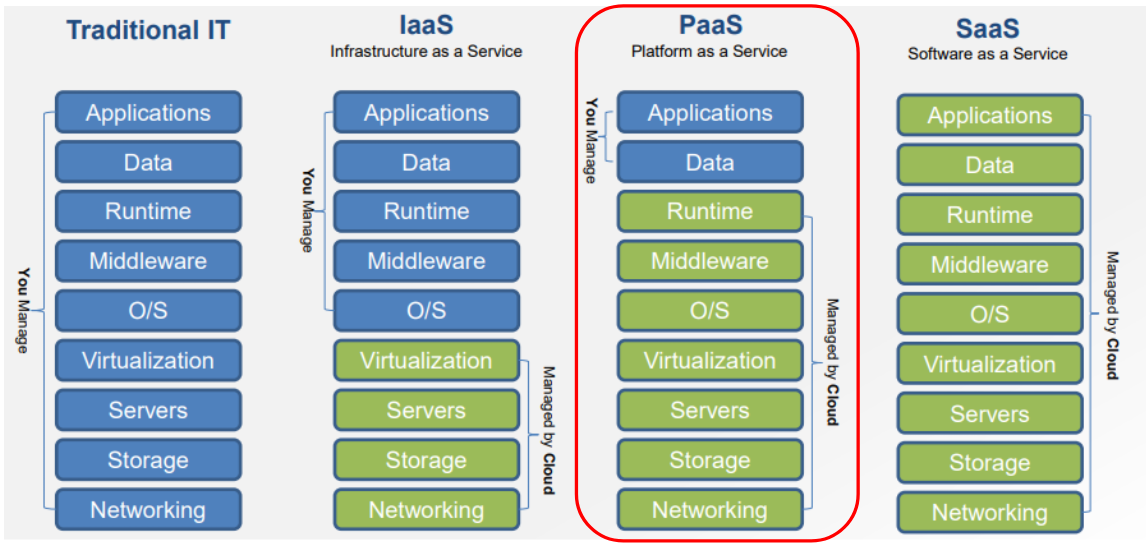
\includegraphics[width=0.8\textwidth]{immagini/Paas.png}
\end{figure}

I PaaS aumentano ancora di più i servizi offerti dallo IaaS offrendoci un intero ambiente di sviluppo e gestione dell'applicazione.\
Vantaggi principali di PaaS per DevOps:\ non è necessario concentrarsi su provisioning, gestione o monitoraggio di elaborazione, archiviazione, rete e software.
\begin{itemize}
    \item Può creare prototipi in \textbf{pochi minuti}.
    \item Può creare nuove versioni o deploy del codice più \textbf{rapidamente}.
    \item \textbf{Self-assemble service}, quindi le varie parti dell'applicazione si assemblano da sole.
    \item \textbf{Scala automaticamente}.
    \item Non bisogna preoccuparci della sicurezza.
    \item Il PaaS si occupa delle strategia di Backup e Recovery.
\end{itemize}

\noindent Il PaaS guadagna meno rispetto a IaaS, al secondo posto per guadagno, e SaaS, al primo posto, ma vale comunque molto:\ circa 19 miliardi di dollari.

\section{Heroku (Paas Freemium)}

È una piattaforma cloud che fornisce una serie di servizi integrati e un intero sistema che ci permette \textbf{non solo di fare il deployment delle applicazioni ma anche di completarle, mandarle in esecuzione e gestirle}.\
Una delle caratteristiche di Heroku è di essere basata su un sistema di \textbf{Container}.\

È nato nel 2007, poi nel 2010 è cresciuto ed è stato acquistato da Salesforce (che si occupa di Saas soprattutto).\
Comprende diversi linguaggi per lo sviluppo del codice (Node, Java, Php, Python, Go, Scala).\

I \textit{Container} di Heroku si chiamano \textbf{Heroku Dynos}.\
Gli Heroku Dynos sono una virtualizzazione, ambienti Linux abbastanza leggeri, isolati che permettono di ``incapsulare'' un'applicazione e tutte le sue dipendenze, librerie\dots\ in un grande ``container''.\
Questo ci permette di spostare la nostra applicazione senza dover dividere le varie parti:\ una volta giunto a destinazione viene prelevata l'immagine del container e ricostruita l'applicazione.\
I Dynos sono utilizzati anche per lo scaling:\ potrebbe volerci un solo Dynos inizialmente, ma poi l'applicazione ingrandendosi avrà bisogno di più spazio e vengono semplicemente aggiunti più container la cui gestione è molto semplice; non dobbiamo più preoccuparci dell'aspetto scalabilità.\

\subsection{Web Dynos}

\begin{figure}[H]
    \centering
    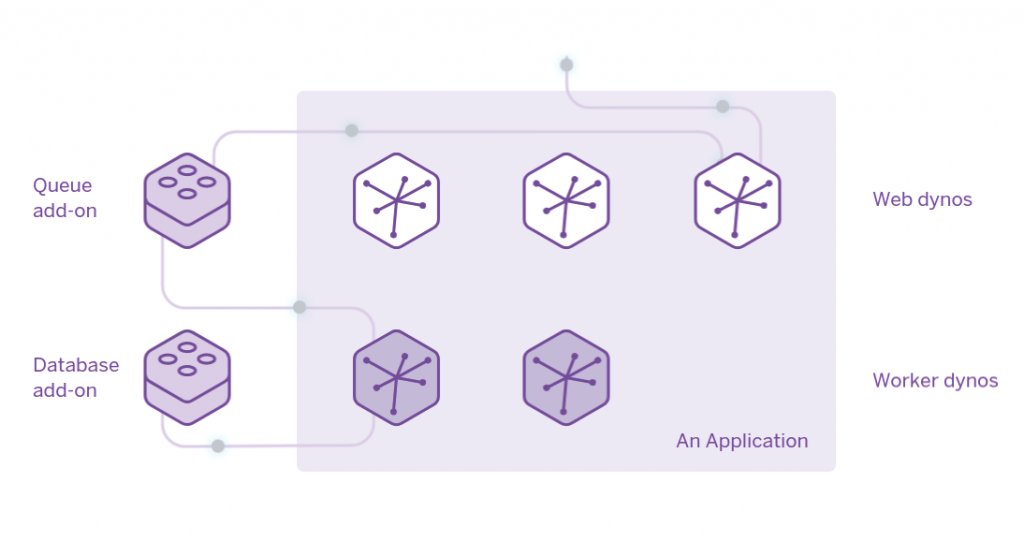
\includegraphics[width=0.9\textwidth]{immagini/Heroku_Dynos.png}
\end{figure}

L'applicazione riceve la richiesta, la richiesta viene inviata a uno degli \textbf{Web Dynos}, viene analizzata e messa in una coda asincrona (che è ottima per la scalabilità orizzontale), poi il \textbf{Worker Dyno} prende la richiesta e la gestisce.\

Se si vuole si può far persistere i risultati \textbf{in un database che è sempre parte di Heroku}.\
In questo caso \textbf{la scalabilità permette di aumentare il numero di Web Dynos} in modo da poter gestire un elevato numero di richieste ricevute contemporaneamente.\
\subsubsection{Buildtime}
Heroku ha bisogno di tre cose per costruire un'applicazione:

\begin{itemize}
    \item Codice sorgente
    \item Lista di dipendenze (Quali sono le cose di cui ha bisogno per funzionare)
    \item Un `\texttt{Procfile}' cioè un file di testo che indica qual è il comando per far partire il codice
\end{itemize}

\begin{figure}[H]
    \centering
    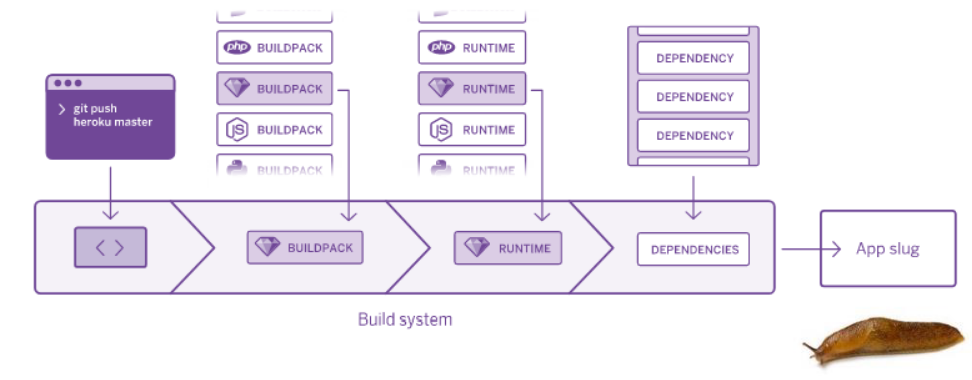
\includegraphics[width=0.9\textwidth]{immagini/Buildtime.png}
\end{figure}
\noindent Queste tre cose fanno parte del Buildtime, cioè la fase di costruzione; una volta date in input parte il \textbf{sistema automatico di built}:\ dopo aver ricevuto il codice scarica il \textbf{Build Packet} (linguaggio, dipendenze, librerie\dots), produce uno \textbf{Slug} e lo mette in esecuzione in un Dyno.\
Il componente finale per eseguire l'applicazione è il sistema operativo (Ubuntu) che è aggiunto da Heroku e che si chiama ``\textbf{stack}''.

\subsubsection{Runtime}
Una volta preparato tutto Heroku crea uno o più Dynos con lo stack e lo slug e fa partire l'applicazione, a quel punto ci abilita a modificare l'app con i vari tipi di Dyno (free, standard, performance, web, workers).

\subsection{Add-ons}
Heroku ha più di \textbf{150 Add-ons} (servizi esterni) da aggiungere alla propria applicazione per estenderne le funzionalità come servizio di autenticazione, log, monitorning, data stores\dots\
Tutto questo attrae l'utente perché offre la possibilità di integrare nuove funzionalità in un tempo molto breve e ne facilita lo sviluppo non dovendo costruire da zero ciò che è richiesto.\

L'aspetto negativo è che questo lega l'utente all'utilizzo della piattaforma e instaura una forma di \textbf{vendor lock-in} rendendo l'applicazione \textbf{difficilmente portabile}.\
Infatti se volessimo spostare la nostra applicazione su un nuovo servizio cloud saremo costretti a rivedere tutto il codice perché gli Add-ons non funzionerebbero.

\section{Microsoft Azure (PaaS e anche IaaS)}
Possiede caratteristiche e capacità che consentono a un'organizzazione di creare o distribuire applicazioni in modo rapido e semplice senza doversi preoccupare dell'OS e dell'infrastruttura sottostanti:

\begin{itemize}
    \item Scalabilità \textbf{verticale}
    \item Supporta \textbf{diversi linguaggi} e ha un'ampia varietà di strumenti per sviluppatori
    \item SQL database
    \item Machine Learning per analisi predittive
    \item Servizi media per supportare video live e on demand
    \item Meccanismi di sicurezza
    \item Data storage (IaaS:\ ai servizi PaaS è spesso richiesto di offrire IaaS)
\end{itemize}

\section{Open Shift (PaaS)}

Il video mostra come si possono ``assemblare'' varie parti per costruire una piccola applicazione che simuli un sistema di voto.\
Il video commerciale sembra molto più semplice di questo, in realtà è abbastanza macchinoso collegare i vari pezzi di funzionalità e linguaggi diversi tra loro.\

\section{Quale PaaS usare?\ Find your PaaS}
In un mercato così variegato è difficile fare la scelta giusta, fortunatamente ci sono dei siti a disposizione che ci permettono di trovare il PaaS adatto alle nostre esigenze semplicemente facendoci scegliere le funzionalità di cui abbiamo bisogno.

\section{Container}

Docker è una piattaforma che ci permette di mandare in esecuzione delle applicazioni software in un ambiente isolato tramite il meccanismo di virtualizzazione dei \textit{containers}.

Nelle macchine virtuali varie applicazioni possono essere eseguite sullo stesso server e ogni VM richiede l'allocazione di risorse (CPU, memoria e storage) e l'installazione del sistema operativo ospite.\
I containers sfruttano la possibilità offerta dal kernel del sistema operativo di eseguire più istanze isolate.\

\begin{figure}[H]
    \centering
    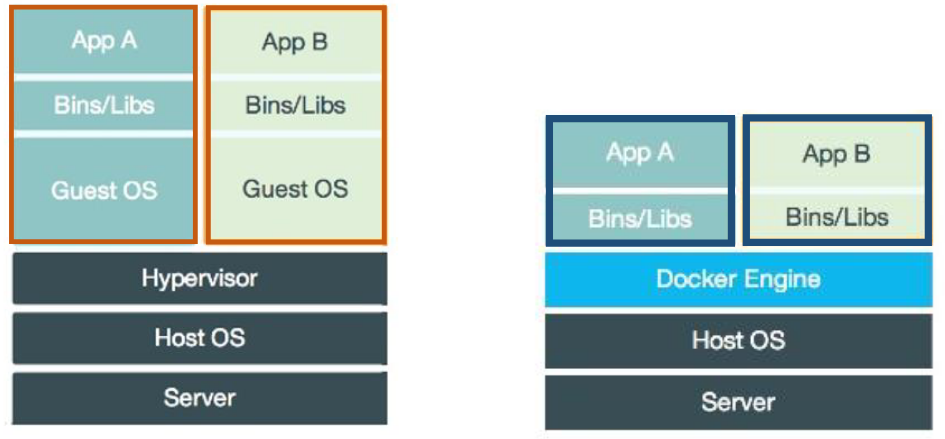
\includegraphics[width=0.7\textwidth]{immagini/Docker_VM.png}
\end{figure}
\noindent Al posto dell'Hypervisor viene montato il Docker Engine.\
In confronto alle VM, i containers sono più leggeri (richiedono meno risorse), più veloci ad avviarsi e più semplici da ``buildare''; tuttavia sono meno sicuri poiché meno isolati.

\subsection{Docker}

Docker sfrutta la virtualizzazione basata su containers per eseguire più istanze guest isolate sullo (stesso) sistema operativo.\
I componenti software sono confezionati in \textbf{\textit{immagini}}, che vengono sfruttate come modelli di sola lettura per creare ed eseguire \textbf{\textit{containers}}; inoltre, è possibile montare \textbf{\textit{volumi}} esterni per garantire la persistenza dei dati.\

\begin{center}
    ``Build, ship and run any app, anywhere.''
\end{center}

\subsubsection{Docker images}
Sono template in sola lettura usati per creare i containers che vengono memorizzati in un Docker \textbf{registry} (pubblico o privato).\
Ogni registry è strutturato in repositories e ogni repository contiene un insieme di immagini per versioni diverse di un software.\
Queste immagini sono strutturate in livelli, ogni livello è a sua volta un'immagine e il livello più basso si chiama \textit{base image}.

\begin{figure}[H]
    \centering
    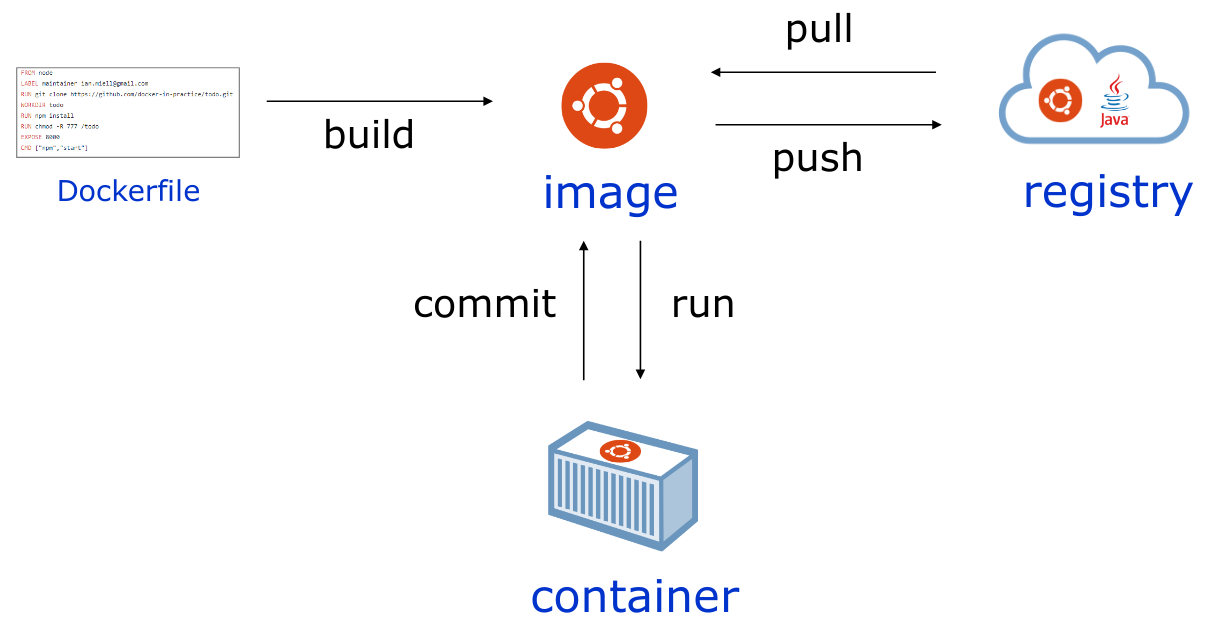
\includegraphics[width=0.8\textwidth]{immagini/docker_cmds.png}
\end{figure}

\subsubsection{Docker compose}

\textit{Docker compose} permette sfruttare più container per costruire applicazioni che consistono di più servizi.

\subsection{Swarm mode}

Docker include la \textbf{\textit{swarm mode}} per la gestione di un cluster di host Docker chiamato \textit{swarm}.

\begin{figure}[H]
    \centering
    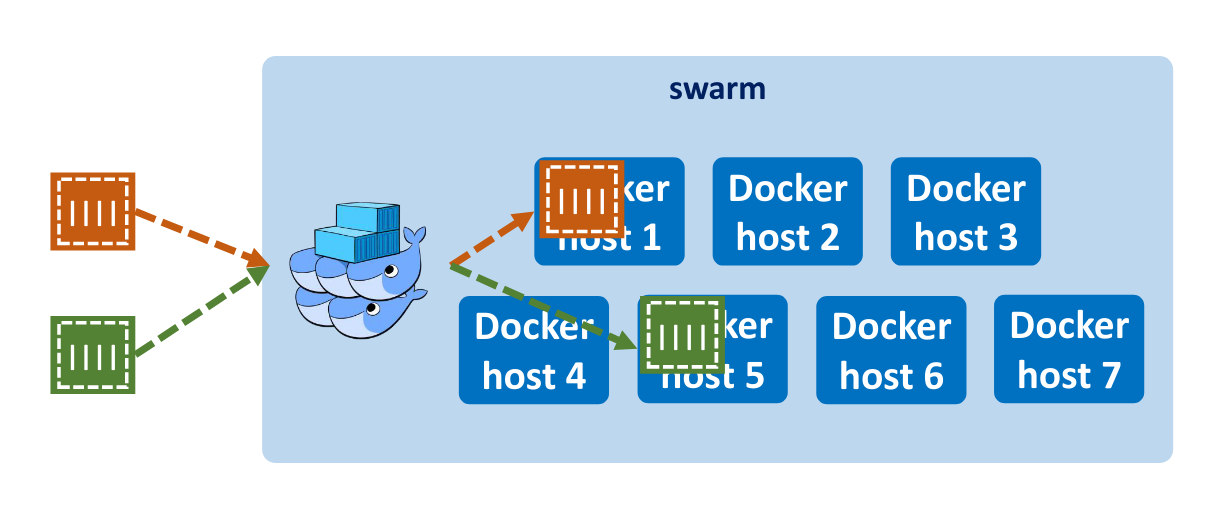
\includegraphics[width=0.8\textwidth]{immagini/docker_swarm.png}
\end{figure}

\noindent I nodi Swarm possono agire come manager, delegando i compiti ai worker, o come worker, eseguendo i compiti loro assegnati.\
È possibile definire lo stato desiderato dei vari servizi nello stack dell'applicazione, incluso il numero di attività da eseguire in ogni servizio.\
I nodi manager assegnano a ogni servizio nello swarm un nome DNS univoco e bilanciano il carico dei container in esecuzione.\
I nodi manager monitorano costantemente lo stato del cluster e riconciliano eventuali differenze tra lo stato effettivo e lo stato desiderato espresso:\ ad esempio, se si configura un servizio per eseguire 10 repliche di un contenitore e una macchina worker che ospita due di queste repliche si arresta in modo anomalo, vengono create due nuove repliche e assegnate ai worker in esecuzione e disponibili.

\subsection{Kubernetes}
Kubernetes è un sistema di orchestrazione per i containers Docker, più esteso di Docker Swarm e che ha lo scopo di coordinare i cluster di nodi su larga scala nella produzione in modo efficiente.

Un \textit{pod} è un gruppo di uno o più containers (ad esempio, contenitori Docker), con archiviazione/rete condivisa e una specifica su come eseguire i containers.\
I contenuti di un pod sono sempre co-localizzati e co-pianificati ed eseguiti in un contesto condiviso.\
Un pod modella un ``host logico'' specifico dell'applicazione:\ contiene uno o più containers dell'applicazione che sono collegati in modo relativamente stretto.\

Il kubelet è l'``agente nodo'' primario che viene eseguito su ogni nodo.

\begin{itemize}
    \item Il kubelet funziona in termini di PodSpec (un oggetto \texttt{YAML} o \texttt{JSON} che descrive un pod).
    \item Il kubelet accetta una serie di PodSpec forniti tramite vari meccanismi (principalmente tramite il server API) e garantisce che i contenitori descritti in quei PodSpec siano in esecuzione e integri.
    \item Il kubelet non gestisce i contenitori che non sono stati creati da Kubernetes.
\end{itemize}

\begin{table}[H]
    \centering
    \begin{tabular}{|p{15em}|p{16em}|}
        \hline
        Docker Swarm                                                              & Kubernetes                                                                                \\\hline\hline
        Simpler to install                                                        & Features auto-scaling                                                                     \\
        Softer learning curve                                                     & Higher fault tolerance                                                                    \\
                                                                                  & Huge community                                                                            \\
                                                                                  & Backed by Cloud Native Computing Foundation (CNCF)                                        \\\hline
        Preferred in enviroments where simplicity and fast development is favored & Preferred for enviroments where medium to large clusters are running complex applications \\\hline
    \end{tabular}
\end{table}
